\chapter{試作2号機:インスタンス認識ハンド}
\newpage

\section{要求仕様}
1号機の課題の中で特に,把持機構の自由度が小さい事と,物体の正確な識別が不可能である問題は実用化の障害となる.
そこで2号機ではこれら2点の課題を克服したロボットハンドを開発する.

ハードウェアとして,1号機では対象に近づきグリップすることをゴールとしたが,実使用を考えると物を持ち帰って次の動作をすることが要求される.そこで2号機では手首機構を重視して,より多彩な動きを実現するためアクチュエータを増やし,把持機構の自由度を上げる必要がある.グリッパとして,指定した点で掴む,またグリッパの中心軸で左右対称に掴む,という動作を可能にする機構が必要である.また,掴む時の把持点決定及び指定した点を掴めるようアクチュエータで調整できることが要求される.そして掴んだ後の物体の滑り防止機構が必要である.
物体をピックアップするために,環境把握に加えて物体との距離を正確に捉える必要がある.

ソフトウェアとして,1号機に搭載したスマートフォンでは環境認識に1秒を要したため,より高速に演算できる計算リソースが要求される.多自由度化に伴いより多くのアクチュエータを制御するため,スマートフォンではなくGPUを搭載したデバイスで学習・推論を行う必要がある.また,1号機では色のみの認識であったが,把持対象物を"物体"として認識し,複数種類に拡張して識別できることが要求される.


\section{機構設計・機体デザイン}
環境把握と対象物との距離を測るためにRGBカメラとデプスカメラを両方搭載したIntel社のRealSenseを用いた.
対象物を持ち上げるために腕に関節を1つ加え,地面から垂直に対象物を挙上できるようにした.
把持中心点を正確に掴むため,2指対立タイプの一般的な形状のグリッパとした.
把持中心位置の制御では,高精度化のためにラック\&ピニオンを用いてサーボモータの回転を水平運動に変換にし,腕を進行方向と垂直な方向にスライドできるようにした.

以上を考慮して\fig{2号機CAD}に示すようなフレームを3DCAD(123D Design Autodesk社を使用)で設計した.また,ロボットハンドの向きは\fig{2号機向き}に示す,ソフトウェアでの画像(配列)の向きと同様の定義とする.

\begin{figure}
    \centering
    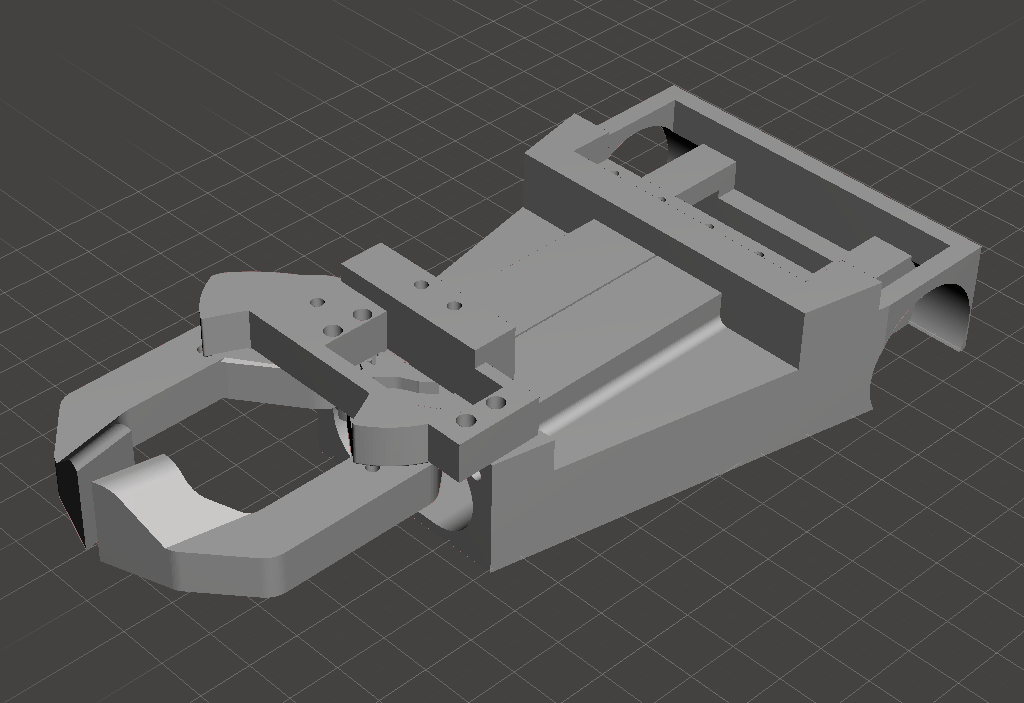
\includegraphics[width=\linewidth]{figure/chapter4/2号機CAD前}
    \caption{3DCAD image of prototype No.2}
    \label{fig:2号機CAD}
\end{figure}

% 向きはここで定義する.CADの写真を使って向きを定義する.

\section{実機作製}

\tab{2号機部品}に2号機作製に当たって使用した部品をまとめた.

\begin{table}[H]
    \centering
    \caption{Components of prototype No.2}
    \begin{tabular}{cc}\toprule
        本体フレーム & PLA(赤) \\
        デプスカメラ & RealSense D435i \\ 
        マイコン & Arduino Nano \\ 
        DCモータ & \href{http://akizukidenshi.com/catalog/g/gM-12379/}{STLギヤモータ 栄42D長軸型} \\ 
        サーボモータ & \href{https://hitecrcd.co.jp/products/servo32225/}{HS-225MG} x1,\href{https://hitecrcd.com/products/servos/discontinued-servos-servo-accessories/hsr-5990tg-hmi-ultra-premium-robot-servo/product}{HSR-5990TG} x1,\href{https://hitecrcd.co.jp/products/servo31422s/}{HS-422} x1 \\ 
        バッテリー & モバイルバッテリー \\ 
        タイヤ & \href{https://tamiya.com/japan/products/70194/index.html}{TAMIYA製スパイクタイヤ} \\
        リニアガイド &  \\
        ラック\&ピニオン &  \\ \bottomrule
    \end{tabular} 
    \label{tab:2号機部品}
\end{table}

1号機と同様にロボットハンドのフレームは簡便さと軽さを考慮して3Dプリンタ(Adventure3)で造形した.
\fig{2号機外観}に作製したロボットハンドの外観を示す.サーボモータを

2号機の総重量は572.27gであった.

\begin{figure}
    \centering
    \begin{minipage}{\linewidth}
        \centering
        \includegraphics[width=\linewidth]{figure/chapter4/2号機外観}
        \caption{Appearance of Prototype No.2. Weight is 572.27 g.}
        \label{fig:2号機外観}
    \end{minipage}
    \begin{minipage}{\linewidth}
        \centering
        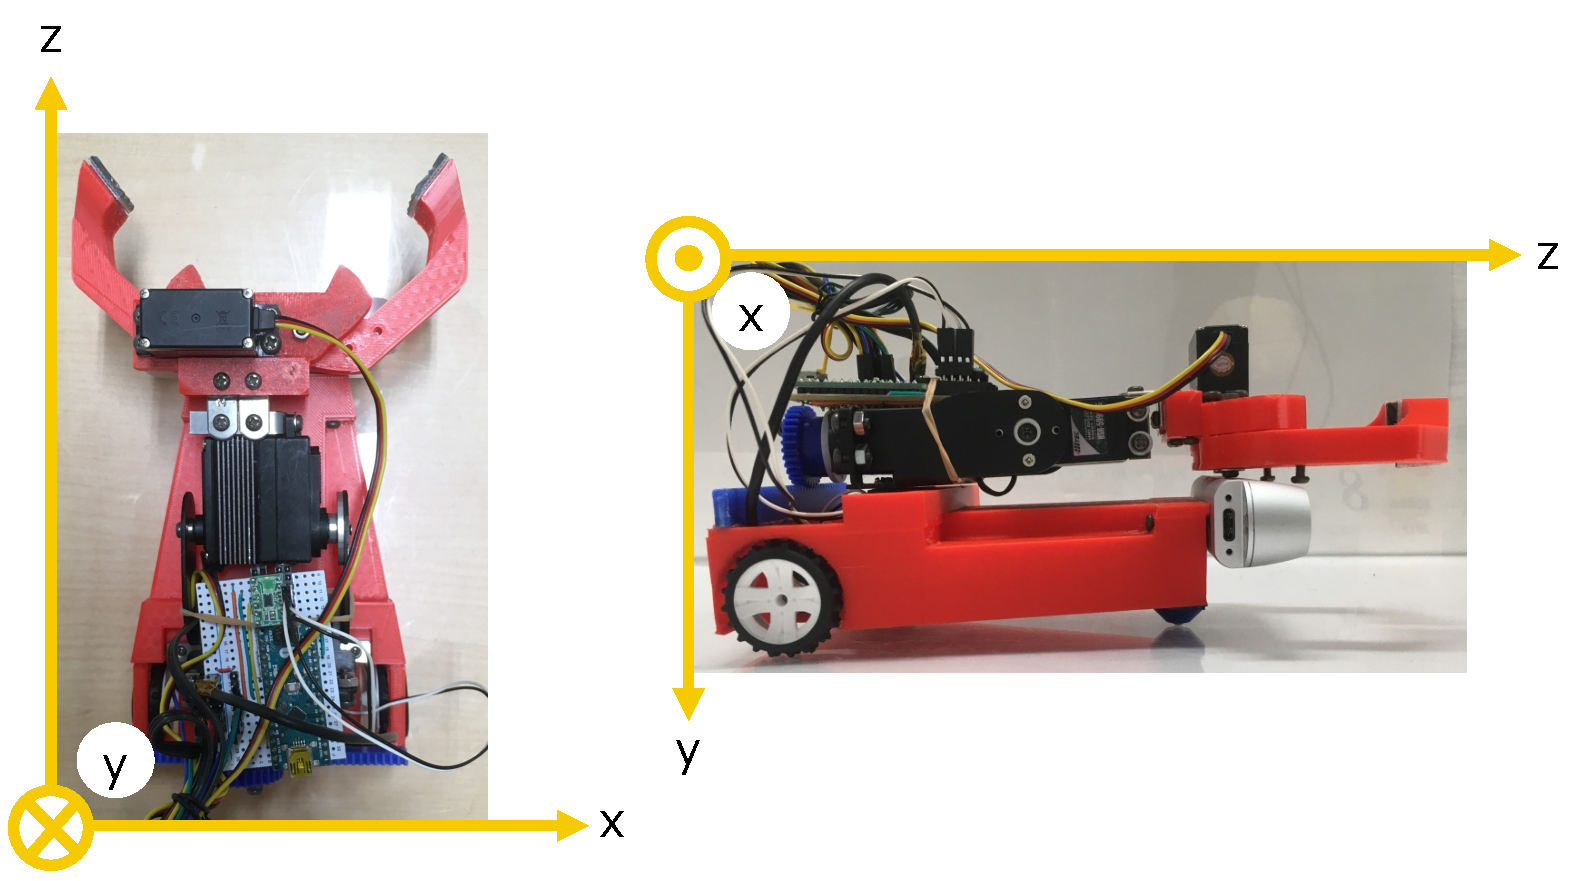
\includegraphics[width=0.9\linewidth]{figure/chapter4/2号機向き}
        \caption{Definition of orientation at prototype No.2}
        \label{fig:2号機向き}
    \end{minipage}
\end{figure}


\section{制御アルゴリズム}
2号機では強化学習ではなく比例制御の考え方を利用した手法及びルールベースによって対象物のピックアップを行う.

接近動作では2段階に分けて行う.まず対象物までのラフな接近について述べる.
対象物のマスクを取得し重心を計算する.その重心がロボットハンドの中心軸に来るように左右輪のスピードをそれぞれ独立に以下の更新式によって制御しながら接近する.

\begin{lstlisting}[caption=接近アルゴリズム, label=code:motor]
    r_motor = (1 - error_distance) / 2 * MAX_SPEED
    l_motor = (1 + error_distance) / 2 * MAX_SPEED
\end{lstlisting}

ここで\texttt{MAX\_SPEED}はモーターの最大スピードで今回は100とした.\texttt{error\_distance}はロボットハンドと対象物との画像内におけるx軸方向のズレを画像の横の長さで規格した値であり,-1から1の値をとる.そして対象物から20cmまで近づいたら停止させる.

次に,対象物の重心にハンドの把持中心が来るように横方向にラックピニオンで修正を加える.この時,画像におけるピクセル間距離を実距離に変換し重心とハンド中心の変位をなるべく小さくするようにサーボを動かす.そしてデプスカメラが対象物に覆われて見えなくなるまで直進する.
そこからさらに4cm直進しグリッパーを閉じる.その後腕を上げ物体を持ち上げ,この際のデプス画像を保持しておく.そこから1秒ごとにデプス画像の現フレームとのピクセル数比を取り,50\%以下であったら失敗とし,5秒落とさず維持したら把持成功とした.

把持が成功したらホームポジションまでコード\ref{code:motor}と同様の制御で戻る.ホームポジションの認識にはARマーカーを使用した.

なお,Arduinoとのシリアル通信では1回に2byteまでしか送信できず,String型でモーター5つの情報を送信すると遅延や読み飛ばしが発生した.そこで2号機ではモーターの取る値をデジタル化し情報を圧縮してByte型で送信するようにした.実際に取る値と送信bit信号の対応表を\tab{2号機信号表}に示す.

\begin{table}
    \centering
    \caption{}
    \begin{tabular}{cccc}\toprule
        Actuator & Bit serial & Value @ Arduino & Value @ Python \\ \midrule
        Forward right DC motor & 000 & 0--100(step 5) & 0--20  \\ 
        Forward left DC motor & 001 & 0--100(step 5) & 0--20 \\ 
        Grip servo & 010 & 0 / 100 & 0 / 1\\ 
        Vertical swing servo & 011 & 0 / 100 & 0 / 1 & 011 \\ 
        Horizontal slide servo & 100 & 0--180 (step 10) & 0--18 \\ 
        Terminate & 101 & 0 / 1 & 0/1 \\ 
        Backward right DC motor & 110 & 0--100(step 5) & 0--20 \\ 
        Backward left DC motor & 111 & 0--100(step 5) & 0--20 \\ \bottomrule
    \end{tabular} 
    \label{tab:2号機信号表}
\end{table}

Bit serialが駆動させるアクチュエータを2進数で示しており,動かす値をValue @ Pythonに示す10進数を5桁の2進数に変換してそれぞれをドッキングして8桁の2進数としてシリアル送信する.


デプスカメラおよびArduinoの制御はG-DEP社のDeepLearning BoxII(Ubuntu16.04)を使用し,計算リソースはNVIDIA社のGPU(TITAN RTX)を使用した.
プログラムは以下のURLの筆者のGitHubで公開している.
\url{https://github.com/yumion/onodera-lab/tree/master/robotHandV2}


\subsection{デプスカメラを使用したカメラ画像内における実距離推定}
把持位置を制御する際,画像内の実際の長さ知る必要がある.そこで,ピクセル間距離から実距離を回帰処理によって求めた.また,カメラから測る対象物までの距離にも依存するため,デプスカメラを用いて距離依存性についても回帰処理を行い,2段階で求めた.

壁に30cm定規を置き,カメラは壁と平行になるよう設置した.壁からカメラの距離$z$(cm)を変えながら定規の目盛りのピクセル座標を取得し,横軸にピクセル差分$\Delta \rm{pixel}$,縦軸にそのピクセルに対応する定規の目盛り幅$\Delta x$(cm)をプロットした(\fig{pix2dist}).また,各$z$で線形回帰を行ったあと横軸に壁からカメラの距離$z$,縦軸に傾き$a$をプロットし線形回帰を行い,全ての距離$z$におけるピクセル間距離を求めた(\fig{depth2grad}).


\begin{figure}[H]
    \centering
    \begin{minipage}{0.45\columnwidth}
        \centering
        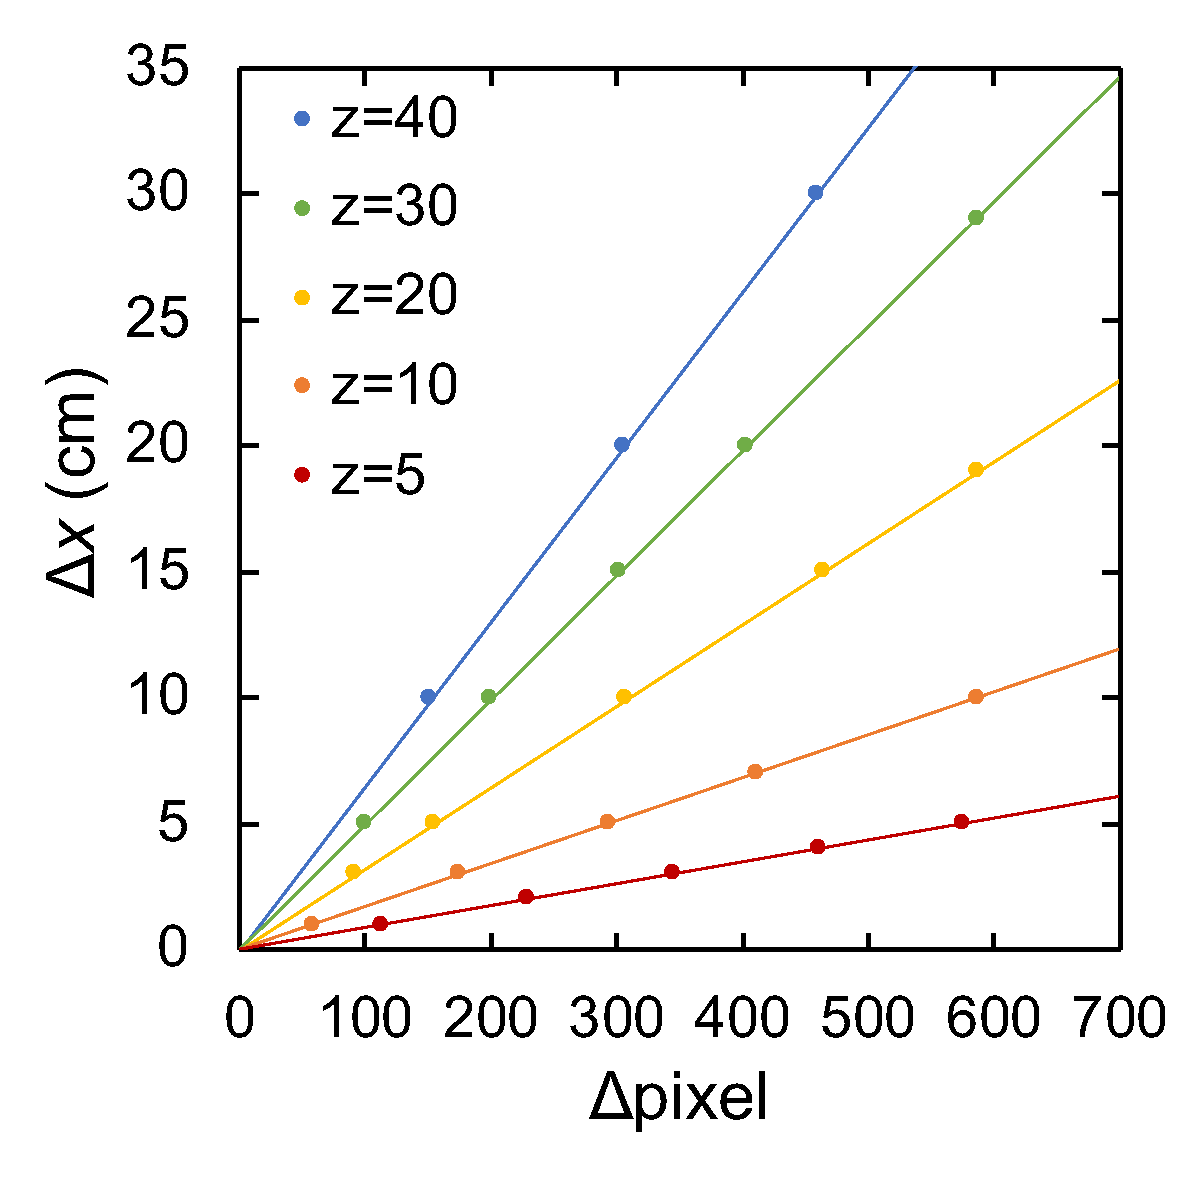
\includegraphics[width=\linewidth]{figure/chapter4/pixel2distance}
        \subcaption{Pixel to Distance}
        \label{fig:pix2dist}
    \end{minipage}
    \begin{minipage}{0.45\columnwidth}
        \centering
        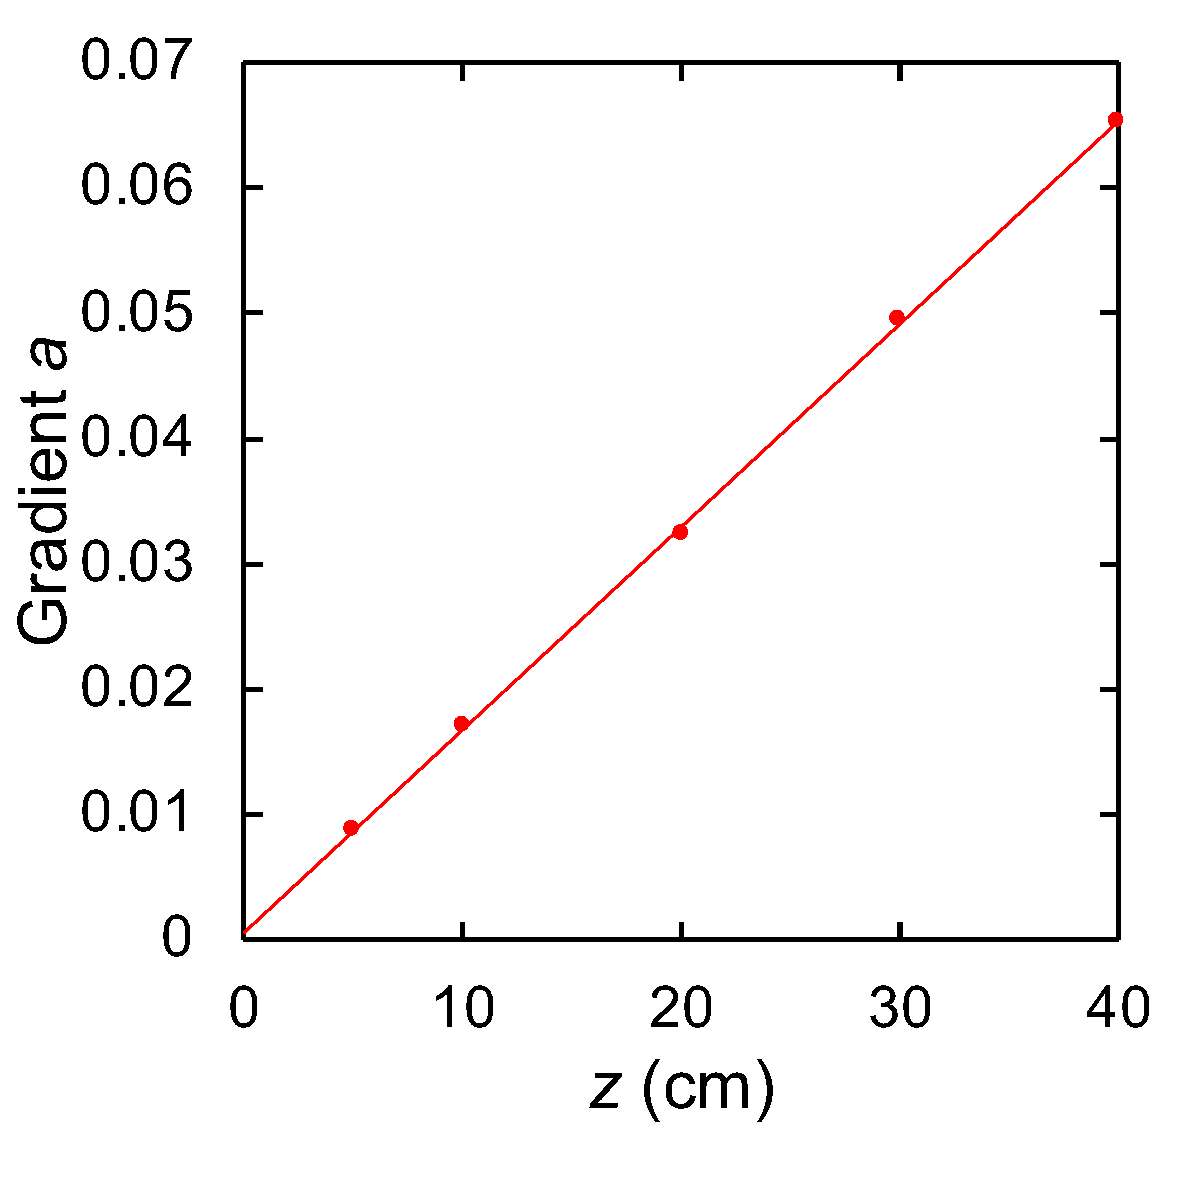
\includegraphics[width=\linewidth]{figure/chapter4/depth2gradient}
        \subcaption{Dependency of depth}
        \label{fig:depth2grad}
    \end{minipage}
    \caption{Convert pixel-wise to distance in real.}
    \label{fig:pix2distance}
\end{figure}


\begin{figure}[H]
    \centering
    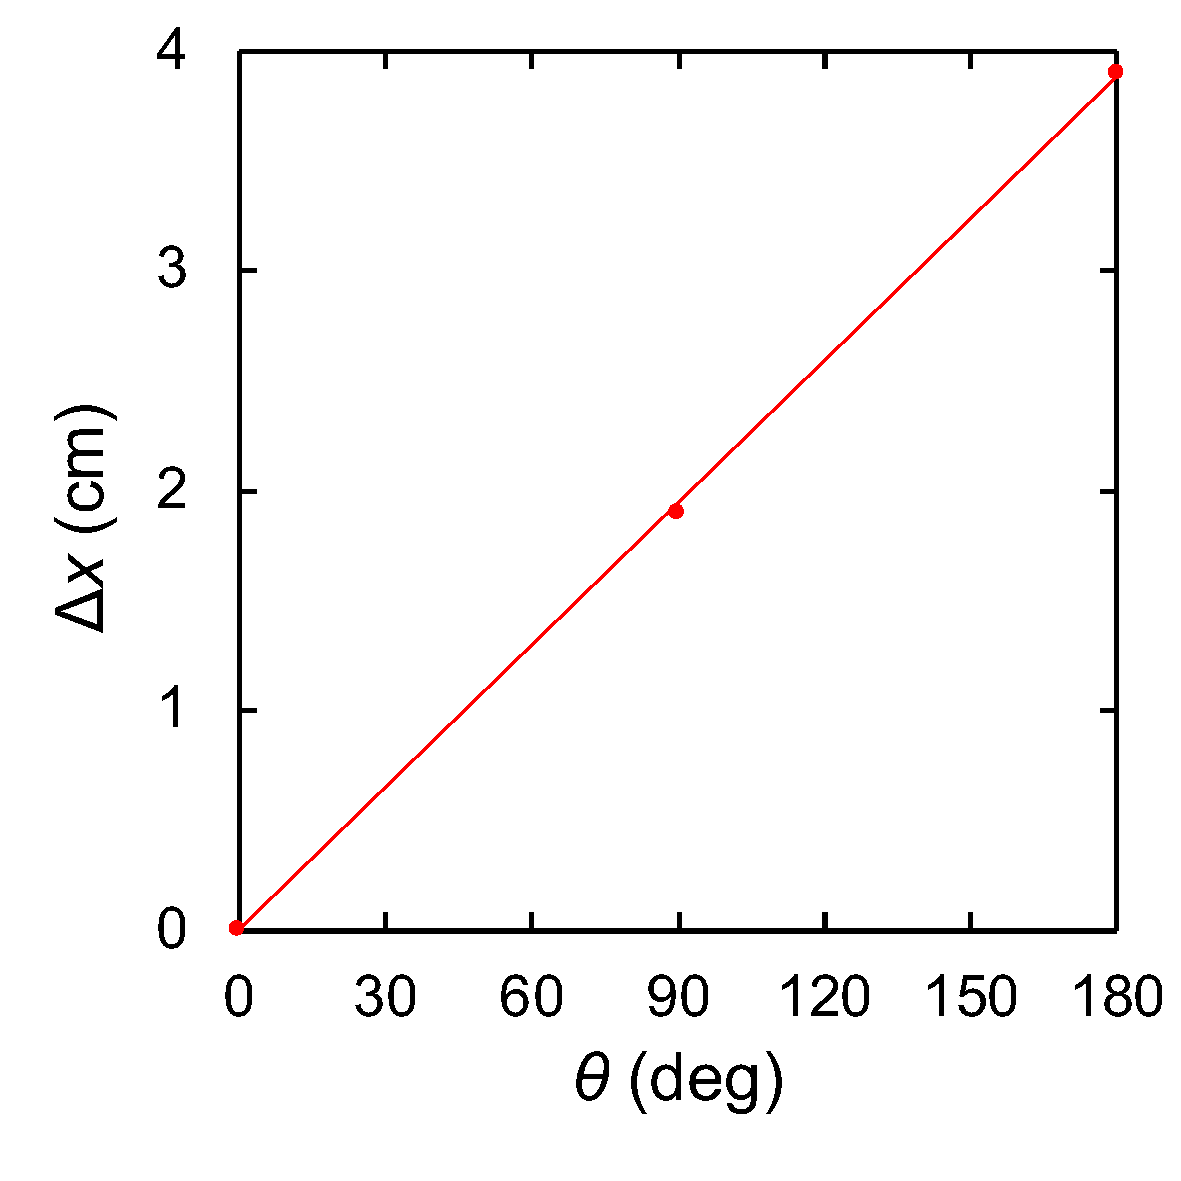
\includegraphics[width=0.5\linewidth]{figure/chapter4/servo2distance}
    \caption{Convert servo input to distance.}
    \label{fig:servo2dist}
\end{figure}

以上から,実距離$\Delta x$はピクセル間距離$\Delta \rm{pixel}$とカメラと対象物の距離$z$を用いて
\begin{align}\label{eq:ピクセル間距離}
    \Delta x \simeq (0.0016z + 0.0006) \cdot \Delta \rm{pixel}
\end{align}
と推定できる.

また,ラック\&ピニオンの回転から水平移動に変換するためには,サーボが0\deg -- 180\deg まで可動するため,その移動最大距離を測定しておき(4cm),各角度における0\deg からの移動量をプロットし線形回帰する(\fig{servo2dist})ことで以下のように求められる.

\begin{align}\label{eq:スライド角度}
    \Delta x \simeq 0.0216 \theta
\end{align}
ここで,$\Delta x$は水平移動距離(cm),$\theta$はサーボの回転角度(deg)である.
\eq{ピクセル間距離}と\eq{スライド角度}から
\begin{align}
    \theta & \simeq \dfrac{\Delta x}{0.0216} \\
           & = \dfrac{0.0016z + 0.0006}{0.0216} \Delta \rm{pixel} \\
\end{align}
として画像からサーボを何度動かせば良いかが分かる.なお,実装上はサーボの可動範囲が0\deg -- 180\deg を考慮して
\begin{lstlisting}[label=code:servo]
    vertical_deg =\
        (max(min(vertical_pos // 0.0216, 90), -90) + 90) // 10
\end{lstlisting}
とすることで入力の最小0,最大を180とし,サーボへの入力が0の時に真ん中である90\deg とし,それを1/10にデジタル化して送信する.\texttt{vertical\_pos}は$\Delta x$(cm),\texttt{vertical\_deg}は$\theta$(deg)である.


\subsection{Mask R-CNNを用いた物体のセグメンテーションと測距}
Instance Segmentationの手法の1つであるMask R-CNNを用いた.MSCOCO2014および2017のデータセットで学習した.
学習した結果を\tab{MSCOCO評価}に示す.

\begin{table}[H]
    \centering
    \caption{Results of Mask R-CNN validated by COCO.}
    \begin{tabular}{ccccc}\toprule
        & \multicolumn{2}{c}{Object Detection} & \multicolumn{2}{c}{Segmentation} \\ 
         & 2014 & 2017 & 2014 & 2017 \\ \midrule
        $\rm{AP}^{\rm{IoU}=0.50:0.95} \u{maxDets=100} @Area=all$ & 0.352 & 0.227 & 0.334 & 0.243 \\ 
        $\rm{AR}^{\rm{IoU}=0.50:0.95} \u{maxDets=100} @Area=all$ & 0.438 & 0.299 & 0.405 & 0.301 \\ 
        FPS & 4.078 & 3.880 & 4.013 & 4.002 \\ \bottomrule
    \end{tabular} 
    \label{tab:MSCOCO評価}
\end{table}

また,デプスカメラを用いて検出した物体の距離も同時に測定した.Mask R-CNNの出力であるマスクの重心を求め,その座標までの距離をデプスカメラで測定した.\fig{maskrcnn例}に学習済みモデルを使用した物体検出およびその物体までの測距の例を示す.

\begin{figure}[H]
    \centering
    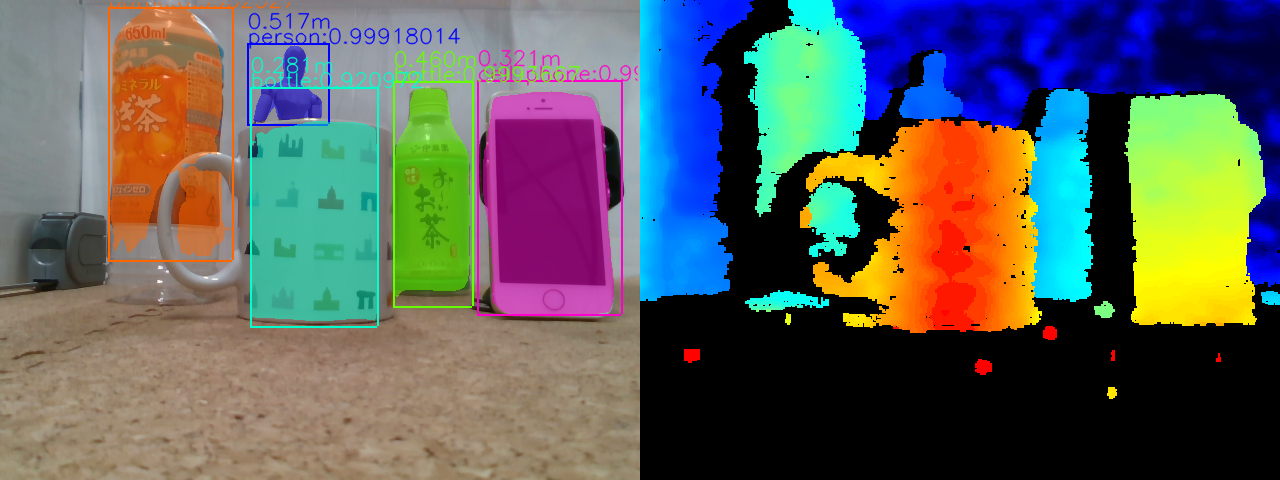
\includegraphics[width=0.7\linewidth]{figure/chapter4/MaskR-CNN_screenshot}
    \caption{Examples of Mask R-CNN inference.}
    \label{fig:maskrcnn例}
\end{figure}


このように,マスクが完璧出なくとも対象物の重心はおおよそ把握できるため,IoUよりもPrecisionを重視し物体検出におけるFPSが高い2014年学習モデルを使う.


\section{評価方法}
今回2号機でアップデートしたのは,対象物の識別と把持動作であったため,この2点に関して評価を行う.

MSCOCOデータセットの中で,机の上にあるものを識別・把持できるかを検証した.
今回,対象とした物体は\fig{対象物}に示す5つの物体(4種類)である.また,\tab{対象物}に各対象物の詳細を示す.
\begin{figure}[H]
    \centering
    
    \begin{minipage}{0.19\columnwidth}
        \centering
        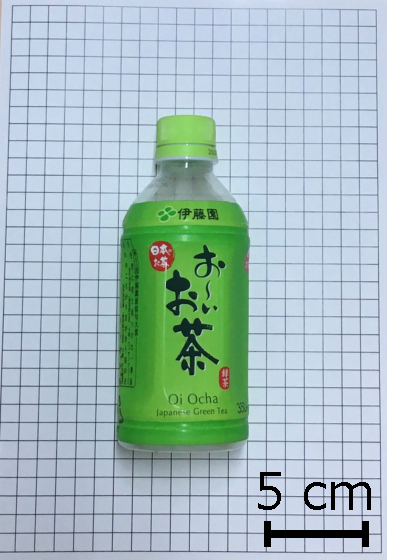
\includegraphics[clip, width=\linewidth]{figure/chapter4/bottle_350ml}
        \subcaption{bottle(350ml)}
    \end{minipage}
    \begin{minipage}{0.19\columnwidth}
        \centering
        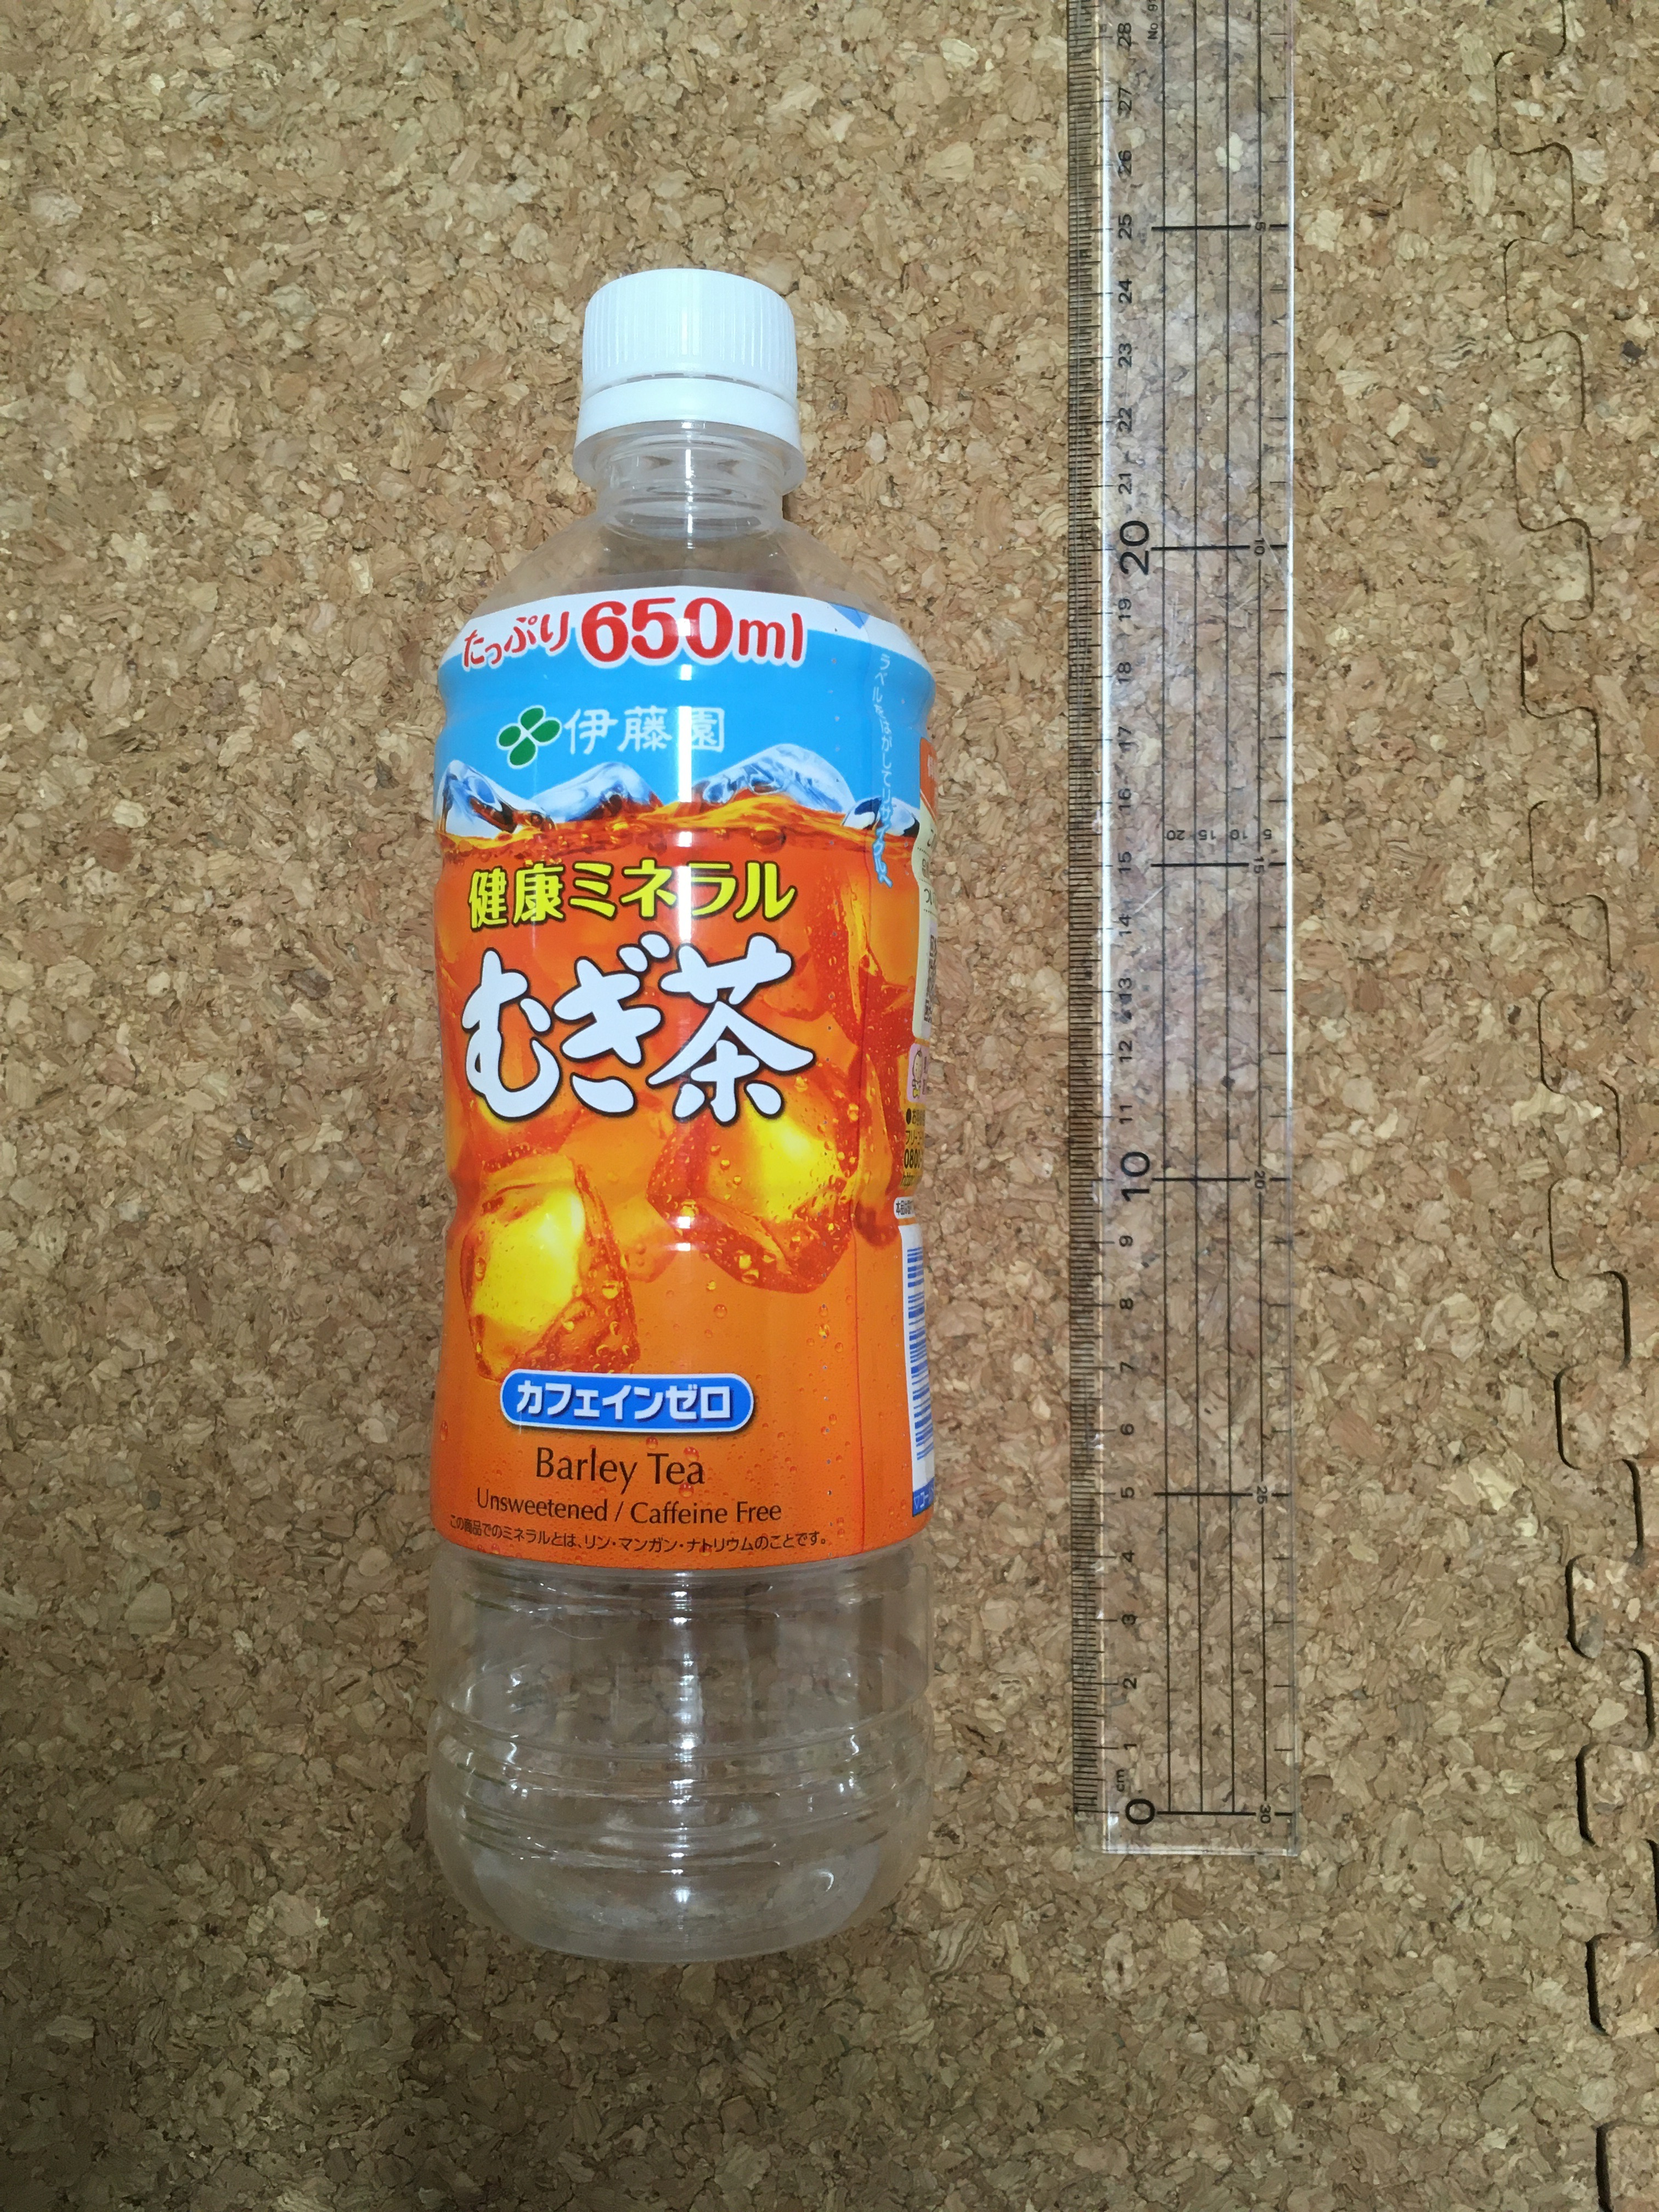
\includegraphics[clip, width=\linewidth]{figure/chapter4/bottle_650ml}
        \subcaption{bottle(350ml)}
    \end{minipage}
    \begin{minipage}{0.19\columnwidth}
        \centering
        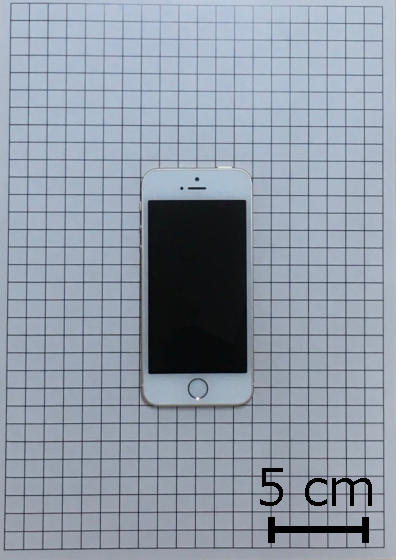
\includegraphics[clip, width=\linewidth]{figure/chapter4/cellphone}
        \subcaption{cell phone}
    \end{minipage}
    \begin{minipage}{0.19\columnwidth}
        \centering
        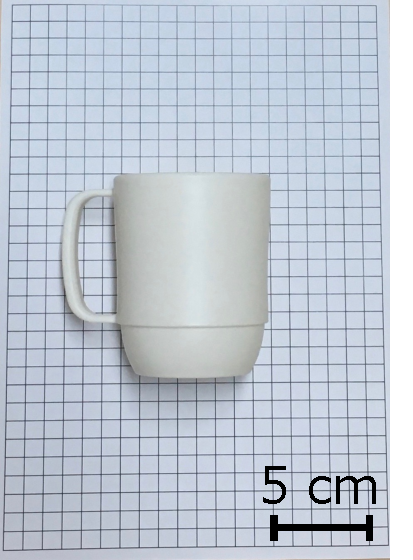
\includegraphics[clip, width=\linewidth]{figure/chapter4/cup2}
        \subcaption{cup}
    \end{minipage}
    \begin{minipage}{0.19\columnwidth}
        \centering
        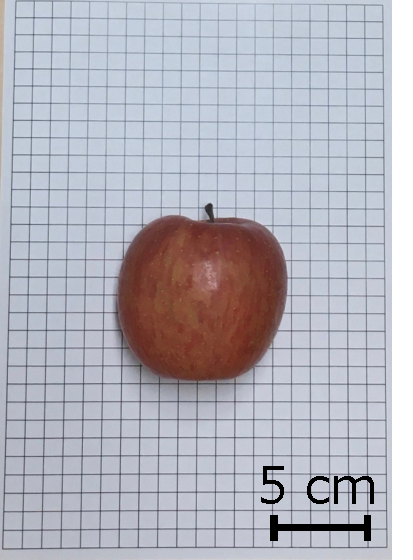
\includegraphics[clip, width=\linewidth]{figure/chapter4/apple}
        \subcaption{apple}
    \end{minipage}

    \caption{Objects.}
    \label{fig:対象物}
    
\end{figure}

\begin{table}[H]
    \centering
    \caption{Details of objects.}
    \begin{tabular}{ccccc}\toprule
        & Size & Weight & \# of Training data & Notes \\ \midrule
        bottle(350 ml) & 16.5 $\times$ $\phi$ 5.9 cm & 26.28 g & \multirow{2}{*}{8880} & Empty \\ 
        bottle(650 ml) & 22.0 $\times$ $\phi$ 6.9 cm & 29.94 g &  & Empty \\ 
        cell phone & 0.78 $\times$ 5.9 $\times$ 12.0 cm & 127.51 g & 5017 & iPhone SE \\ 
        cup & 9.8 $\times$ $\phi$ 7.9 cm & 82.50 g & 9579 & Empty \\ 
        apple & $\phi$ 8 cm & 263.32 g & 1662 & Raw \\ \bottomrule
    \end{tabular}
    \label{tab:対象物}
\end{table}

まず,学習済みモデルを使用してMask R-CNNの識別精度を検証した.また各対象物において,ロボットハンドとの距離すなわち画角によってMask R-CNNの検出精度およびそのクラス分類の精度が異なるかを検証した.

次に,各物体に対して接近成功率および把持成功率を検証した.接近成功率とは,対象物の17cm以内に近づきかつ対象物を正面に捉えて静止したら成功,対象物の正面で止まれなかったら失敗とし,10回試行したときの成功率とする.把持成功率とは5秒間持ち上げ続けたら成功,そうでなければ失敗とし,10回試行したときの成功率とする.
接近および把持のタスクは以下のように定めた.タスク1が接近タスクでタスク2が把持タスク,タスク1+タスク2が接近・把持の一貫タスクである.
\begin{itemize}
    \item タスク1\\
    離れたところに対象物を置き,17cm以内まで接近する.
    \item タスク2\\
    対象物の向かい17cmの場所から把持を行う.
    \item タスク1+タスク2\\
    離れたところに対象物を置き,17cm以内まで接近し,そこから把持を行う.
\end{itemize}


\section{結果}
\subsection{識別性能評価}
"bottle"はどの向きにおいても検出できた."cell phone"はエッジ部分だけでは検出できず,画面側か背面のみ検出できた."cup"は取っ手が写っている角度では検出できたが,取っ手が写らない向きになると"bottle"と誤認識することがあった."apple"はどの向きにおいて認識できなかった.

各対象物において,識別精度の対象物依存性を\fig{mrcnn距離}に示す.なお,"apple"は全ての場所・向きにおいて認識できなかったため載せていない.
\begin{figure}[H]
    \centering
    \begin{minipage}{0.45\columnwidth}
        \centering
        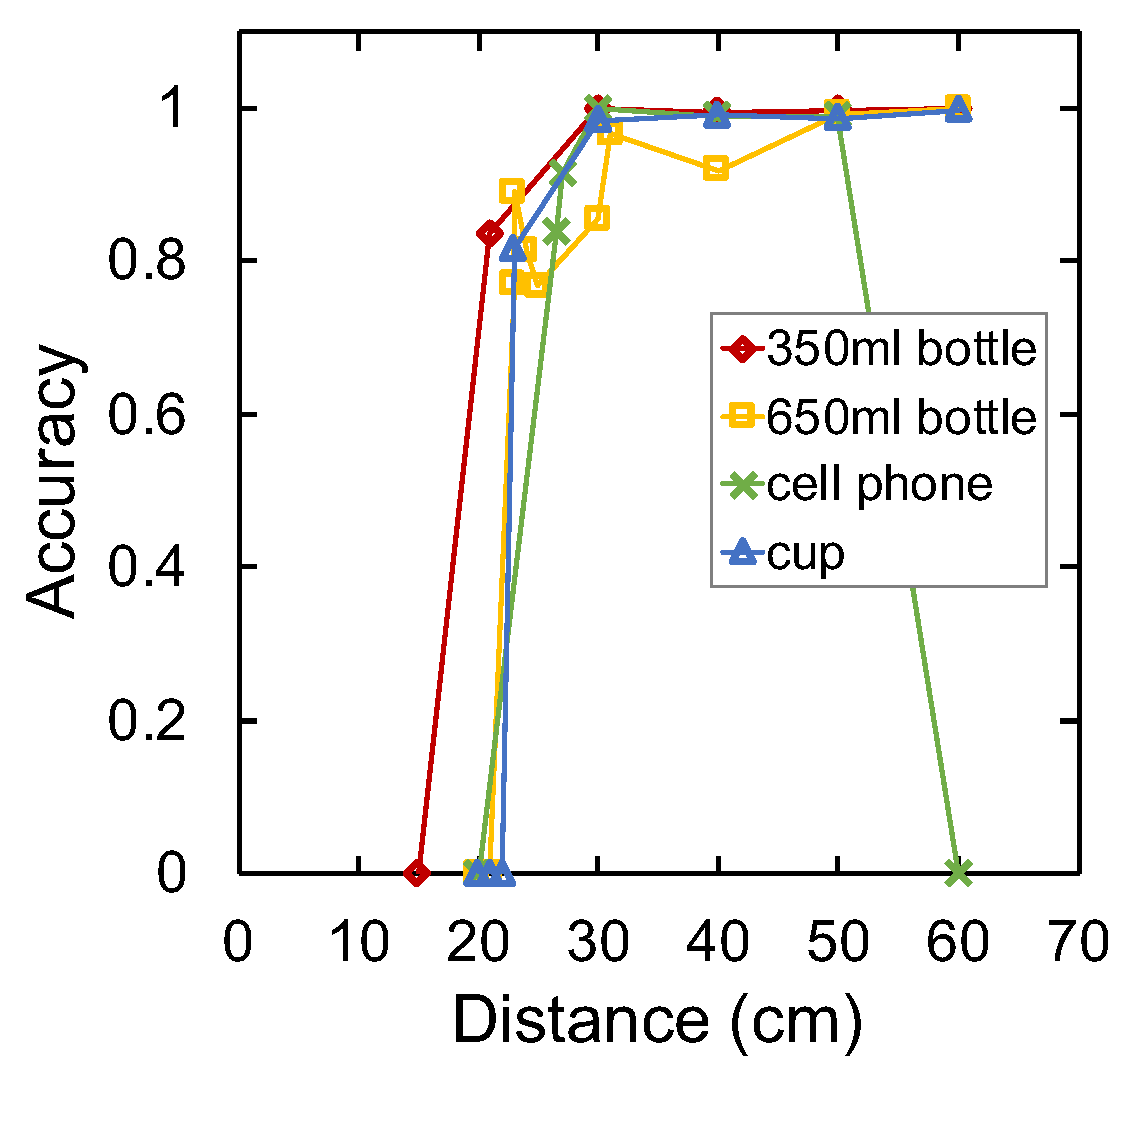
\includegraphics[width=0.95\linewidth]{figure/chapter4/mrcnn_depth}
        \subcaption{Input raw image.}
        \label{fig:mrcnn距離そのまま}
    \end{minipage}
    \begin{minipage}{0.45\columnwidth}
        \centering
        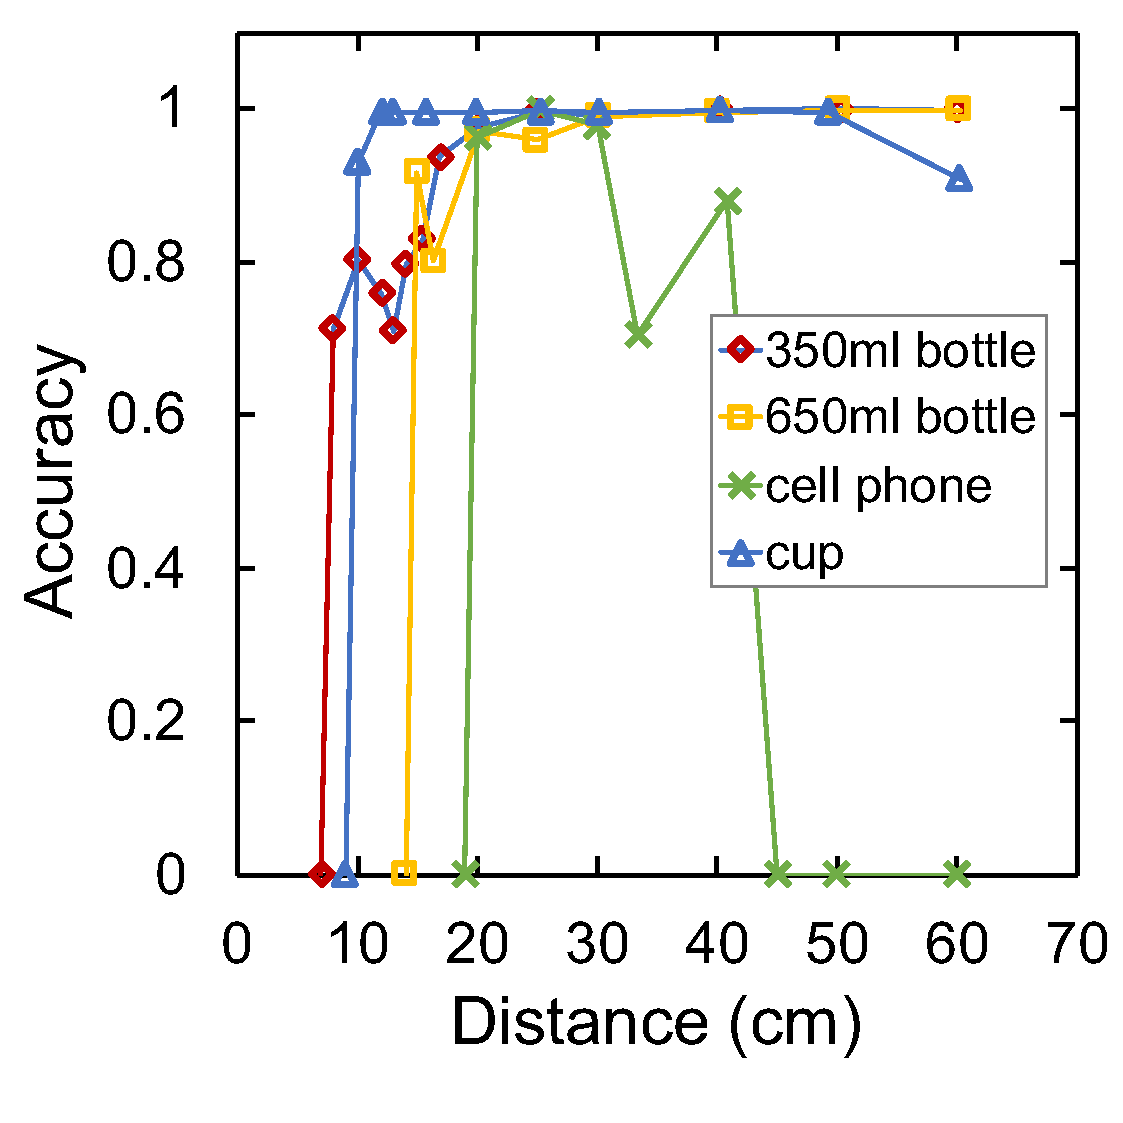
\includegraphics[width=0.95\linewidth]{figure/chapter4/mrcnn_depth_padding}
        \subcaption{Input zero padding image.}
        \label{fig:mrcnn距離パディング}
    \end{minipage}
    \caption{Dependency of distance between camera and object.}
    \label{fig:mrcnn距離}
\end{figure}
入力にカメラ画像をそのまま入れた結果が\fig{mrcnn距離そのまま}であった.30cmを境に識別精度が落ちていることが分かる.

\subsection{把持タスク評価}


\begin{table}[H]
    \centering
    \caption{Success rate on grasping objects tasks.}
    \begin{tabular}{cccc}\toprule
        Objects & Task1 & Task2 & Task1 + Task2 \\ \midrule
        bottle (350 ml) & 60\% & 90\% & 50\% \\
        bottle (650 ml) & 60\% & 80\% & 50\% \\
        cell phone & 60\% & 50\% & 40\% \\ 
        cup & 70\% & 50\% & 30\% \\ \bottomrule
    \end{tabular} 
    \label{tab:把持成功率}
\end{table}

失敗例は,掴み方が悪く掴んでも落とした,掴んで持ち上げたがロボットハンド自体が横転した,持ち上げたがズレ落ちた,などがあった.

また,ホームポジションに戻る動作も実装した.


\section{考察}
appleが認識できなかった原因は,学習データ数の偏りにあると考えられる.\tab{対象物}に示したように,appleだけ他の対象物よりも訓練データが3分の1以下と少ない.したがって今回使用したモデルはappleの認識が弱いモデルだったと考えられる.

Mask R-CNNの検出精度における対象物との距離依存性では,対象物の高さに関係なく30cmから精度が落ち始め,20cmでは全ての物体で検出できなくなった(\fig{mrcnn距離そのまま}).背の高いbottle(650ml)は,距離が近いと画像内に物体全体が収まらず検出精度が下がると予想できるが,背の低いcupも同じように精度が下がった.これは学習データに大きく写っている画像が無いことが原因と考えられる.
そこで,入力画像をzero paddingして対象物を小さく写るようにして入力した結果が\fig{mrcnn距離パディング}である.paddingをすることで大幅に距離依存性が改善され,17cmまで近づいても検出されるようになった.したがって,接近タスクでは17cmを閾値としてそこまで近くタスクとした.

把持成功率より接近成功率が低い原因は,2号機のRGBカメラの位置だと考えられる.2号機に搭載したカメラRealSenseは左端にRGBカメラ,真ん中右寄りにDepthカメラが付いているため,RGB画像は右側を見ることが難しい.そのため,ロボットハンドから距離が離れていれば問題ないが,物体がロボットハンドに近い位置で右側にいると死角となり,認識できないため接近できないという事になる.また,cell phoneとcupは把持成功率が低く,bottleの把持成功率が高い理由としては,把持対象物の対称性だと考えられる.bottleは円筒対称であるため,どの角度からアプローチしても同様の持ち方で把持が可能だが,cell phoneやcupはbottleより対称性が悪いため,ルールベースでは正しい位置で把持できない.これは各物体に対して把持位置を学習するなど,高度なアルゴリズムが必要となる.

\section{まとめ}
物体の種類を識別し,把持し,元いた位置に運搬することができた.



